% !TEX root = JKPS_TeX_sample_eps.tex

\section{Results} %discussion?
\label{sec:results}

To have more quantitative comparisons, associated yields of long-range ($2<|\deta|<4$) near-side correlation functions are calculated by integrating one-dimensional correlation functions over the region $|\dphi|<|\dphi_{\rm{min}}|$:
\begin{equation}
   Y^{\rm{assoc}} = \int_{|\Delta \varphi| < |\Delta \varphi_{\mathrm{min}}| } \mathrm{d} \Delta\varphi \left( \frac{1}{\it{N}_{\rm{trig}}} \frac{ \rm{d}\it{}N_{\rm{pair}} }{ \mathrm{d}\Delta\varphi } - C_{\rm{ZYAM}} \right), 
\end{equation}
where $\dphi_\mathrm{min}$ is the \dphi value from the ZYAM method. 
The left panel of Figure~\ref{fig:ay} shows the associated yield of long-range near-side correlation functions as a function of \Nch for charged hadrons in $1<\pt<2~\mathrm{GeV}/c$, and the multiplicity \Nch is calculated with charged hadrons in $|\eta|<2.4$ and $\pt>0.4~\mathrm{GeV}/c$.
Note that associated yields with initial charged hadrons directly produced from partons are also calculated in the same \Nch bins with final charged hadrons to use same events for associated yields with initial and final hadrons.
The associated yields from \pythia events with the default configuration (red lines) are zero for the entire \Nch range. 
In case of the string shoving model (blue lines), significant amount of associated yields are observed at the entire \Nch range, and it increases with charged hadron multiplicity.
The larger associated yields of initial hadrons than those of final hadrons may indicate that the long-range correlation built from the string shoving smears out through particle decay processes.

\begin{figure}[!h]
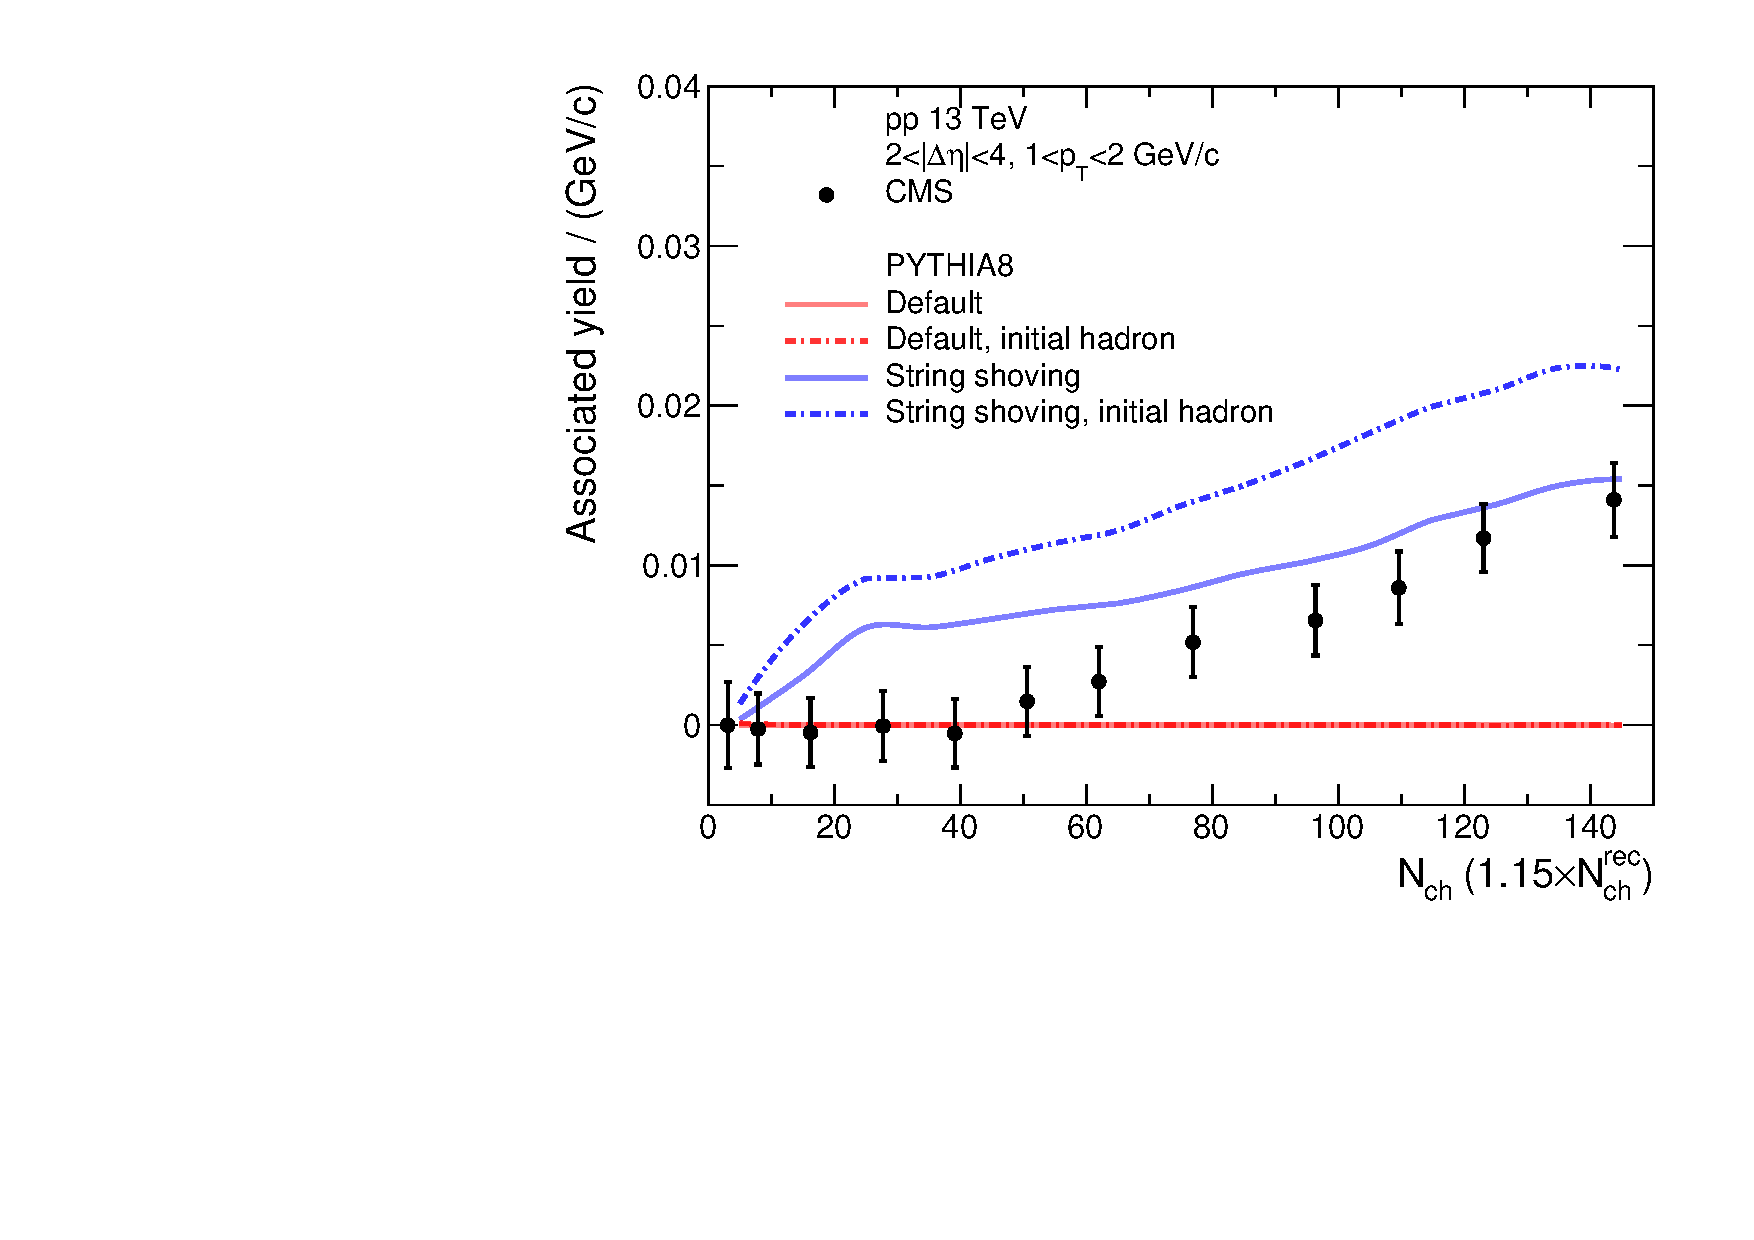
\includegraphics[width=0.49\textwidth]{figures/cmsmult.pdf}
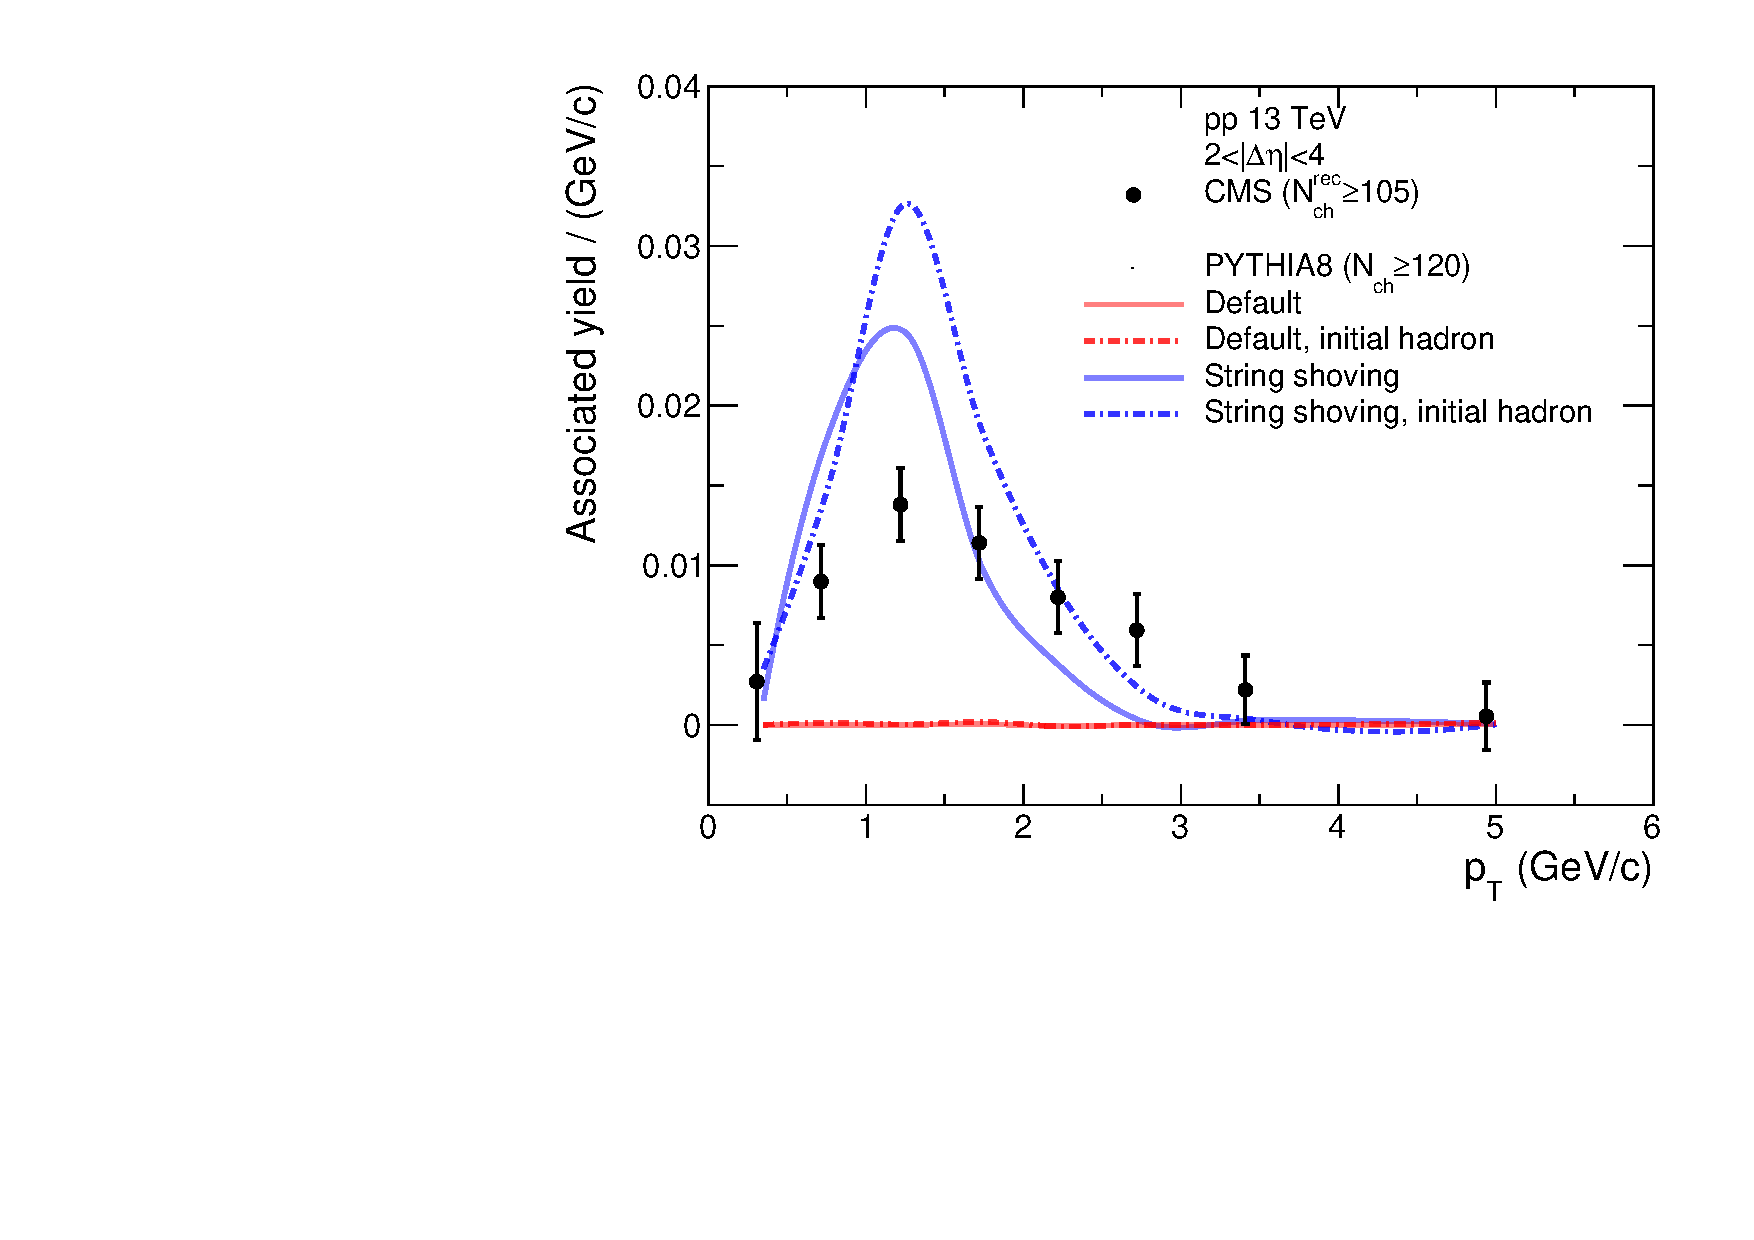
\includegraphics[width=0.49\textwidth]{figures/cmspt.pdf}
\caption{Associated yields of long-range near-side correlation functions as a function of \Nch for charged hadrons in $1<\pt<2~\mathrm{GeV}/c$ (left) and as a function of \pt for high multiplicity events (right). The results from \pythia events with the default configuration and the string shoving model are compared with CMS results~\cite{Khachatryan:2015lva}.}
\label{fig:ay}
\end{figure}

The CMS results~\cite{Khachatryan:2015lva} are compared with the string shoving model.
Note that the CMS results are as a function of the number of reconstructed charged particles ($N_\mathrm{ch}^\mathrm{rec}$), the CMS results are shifted along the $x$-axis ($1.15\times N_\mathrm{ch}^\mathrm{rec}$) based on the reported track reconstruction efficiency.
The associated yields of final hadrons from the string shoving model agree with the CMS result in high multiplicity events ($\Nch>120$), but it overestimates associated yields in lower multiplicity events, indicating that there is a long-range correlation from jets in the string shoving model.
For a more detailed comparison, associated yields as a function of \pt in high multiplicity events are shown in the right panel of Figure~\ref{fig:ay}.
Although the associated yields for charged hadrons in $1<\pt<2~\mathrm{GeV}/c$, shown in the plot as a function of \Nch, are comparable between the string shoving model and the CMS result, they show a different \pt dependence.
The associated yields from the string shoving model is higher than the CMS result around $\pt=1~\mathrm{GeV}/c$, and it drops more rapidly for $\pt>2~\mathrm{GeV}/c$.


\begin{figure}[!h]
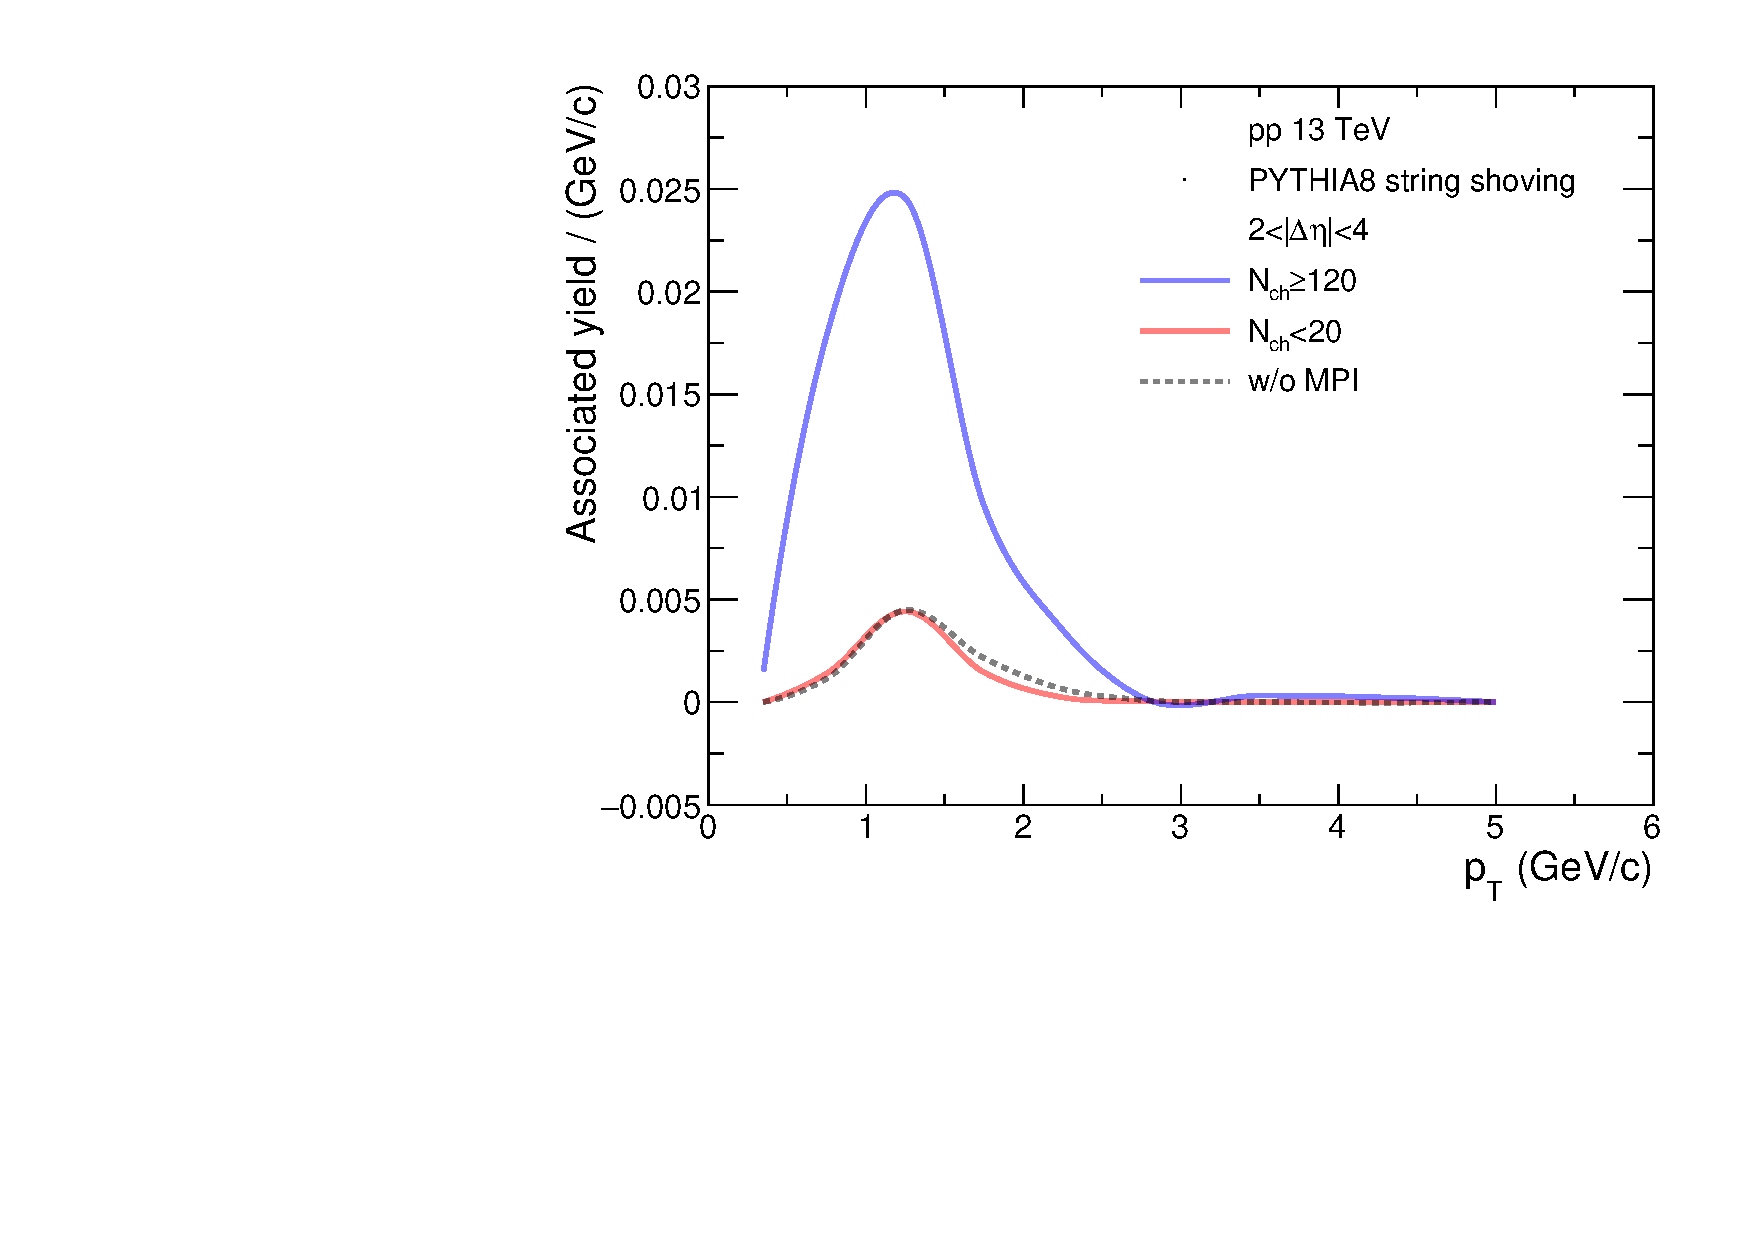
\includegraphics[width=0.5\textwidth]{figures/mpi2.pdf}
\caption{Associated yields of long-range near-side correlations as a function of $\pt$ in \pythia with the string shoving model for low, high multiplicity events (solid lines), and events without multi-partion interaction (dashed line). }\label{fig:wompi}
\end{figure}

For further investigation on the non-zero associated yields from the string shoving model in low multiplicity events ($N_\mathrm{ch}\lesssim 50$), we generated \pythia events with the string shoving configuration but turning off the multi-parton interaction option, so charged hadrons are mostly produced from hard scattered partons.
In these events where the number of strings is expected to be small, a clear long-range near-side correlation is still observed.
Figure~\ref{fig:wompi} shows associated yields of long-range near-side correlations as a function of \pt for different event classes.
Solid lines are from normal low ($\Nch<20$) and high ($\Nch \geq 120$) multiplicity \pythia events with the string shoving configuration, and the dashed line is from events without multi-parton interaction.
The associated yields in normal low multiplicity events and events without multi-parton interaction are consistent. 
This indicates that the strong shoving model introduces a long-range correlation for particles associated with jets, which is not observed in experimental results.


\begin{figure}[!h]
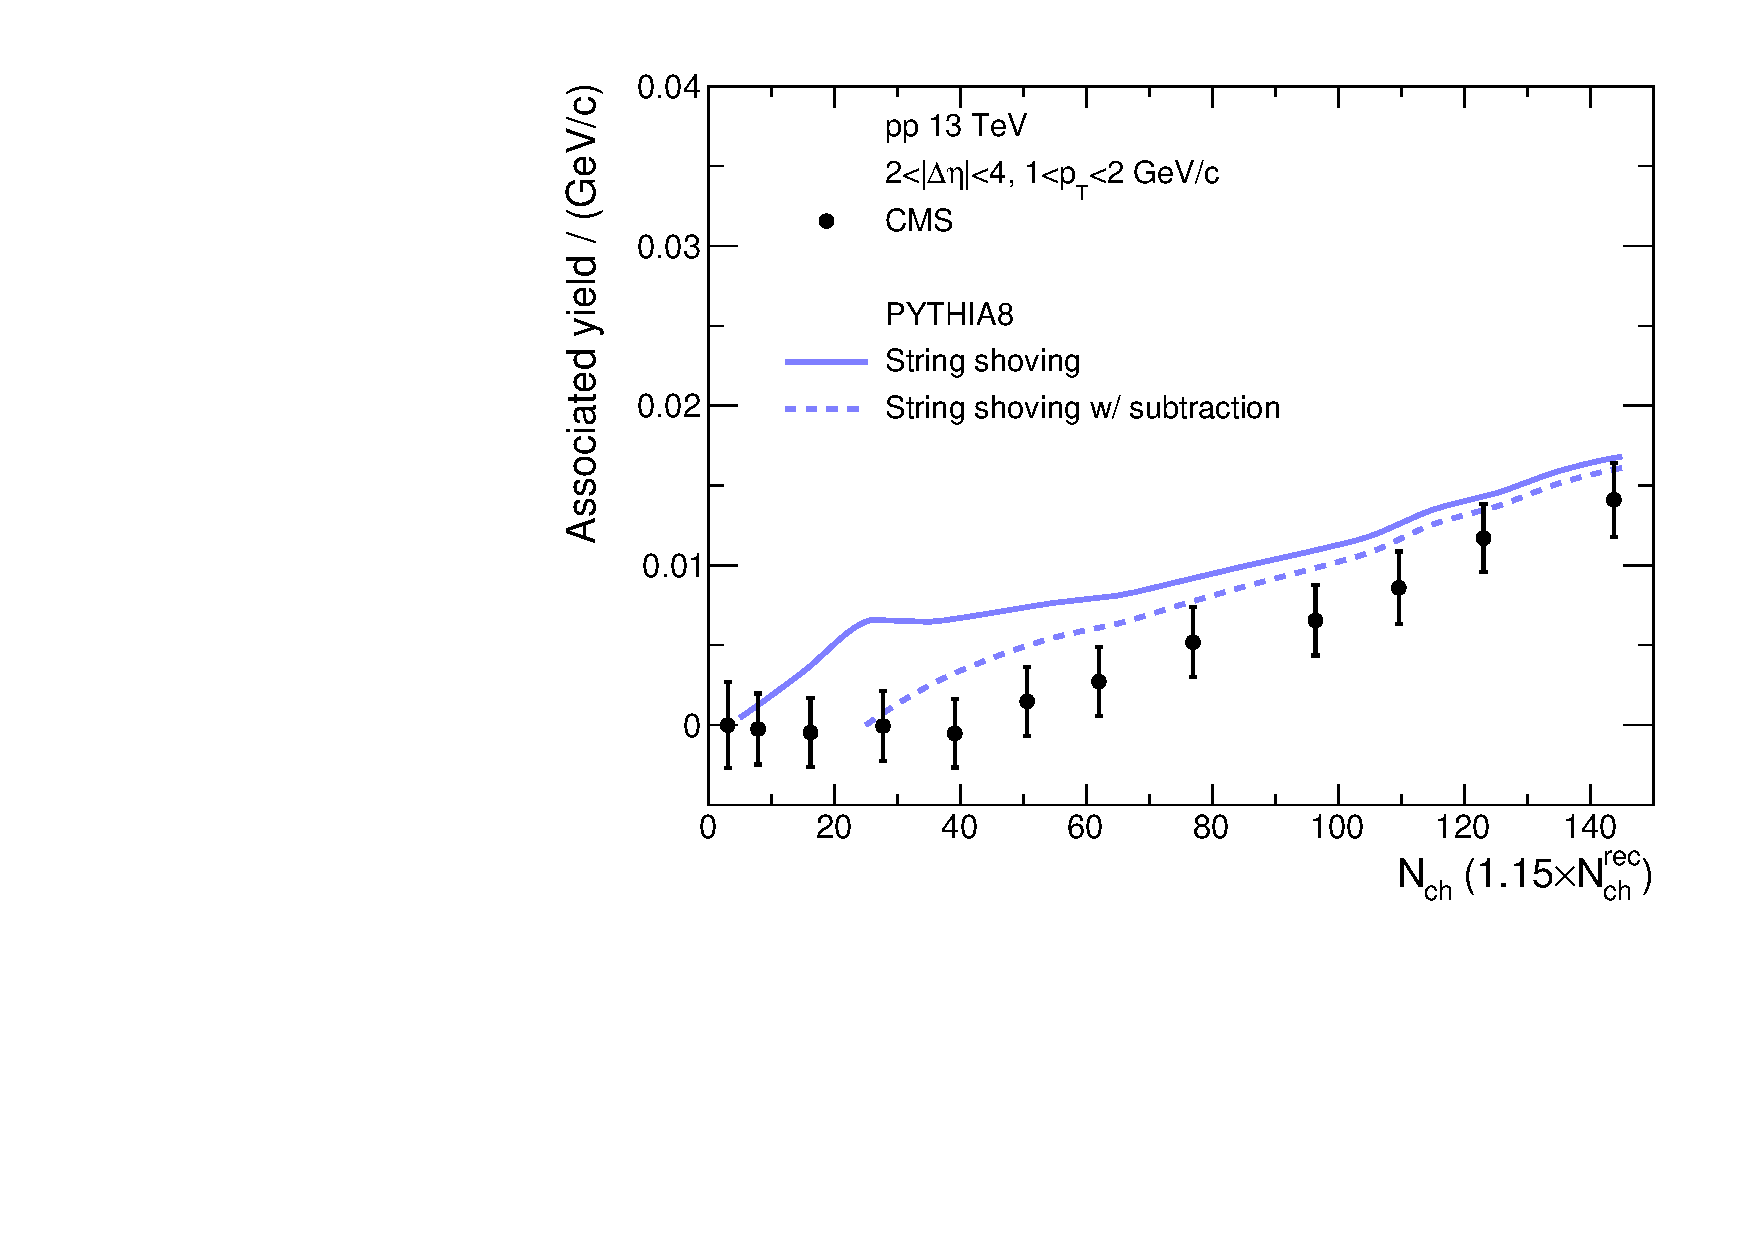
\includegraphics[width=0.49\textwidth]{figures/cmsmultSub.pdf}
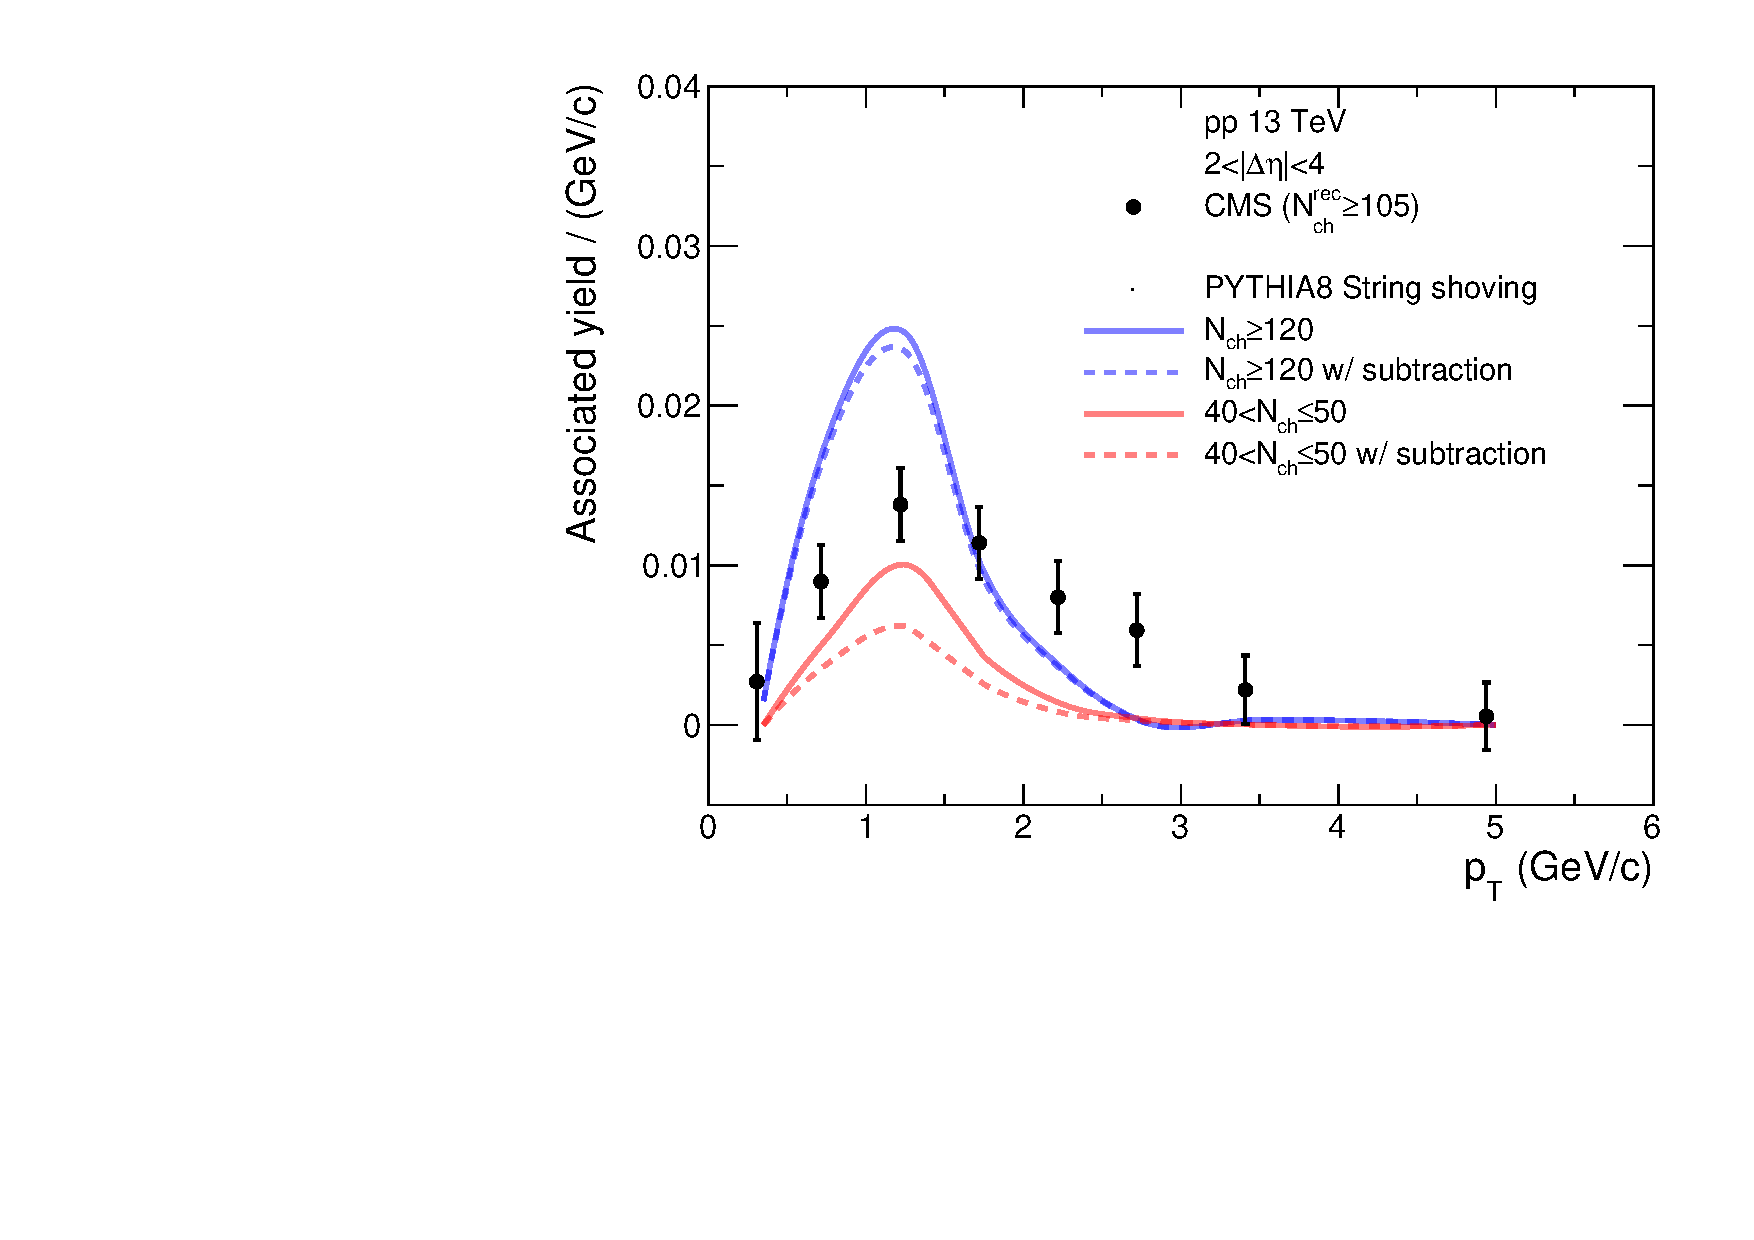
\includegraphics[width=0.49\textwidth]{figures/cmsptSub.pdf}
\caption{Associated yields of long-range near-side correlation functions as a function of \Nch for charged hadrons in $1<\pt<2~\mathrm{GeV}/c$ (left) and as a function of \pt for different multiplicity bins (right). Associated yields in $20\leq\Nch< 30$ are used for the subtraction procedure.}\label{fig:aysub}
\end{figure}

We perform a further analysis to subtract associated yields from jets to have a better comparison with the data.
One simple assumption is that there are two sources of particles, jets and bulk, and there is no correlation between one particle from jets and the other particle from bulk. In such case, long-range two-particle correlation functions after the ZYAM procedure can be expressed as
\begin{align}
    \frac{1}{N_\mathrm{trig}} \frac{\mathrm{d} N_\mathrm{pair}}{\mathrm{d} \dphi} = \frac{1}{N_\mathrm{trig-j} + N_\mathrm{trig-b}} \left( \frac{\mathrm{d} N_\mathrm{pair-j}}{\mathrm{d} \Delta \varphi} + \frac{\mathrm{d} N_\mathrm{pair-b}}{\mathrm{d} \Delta \varphi} \right),
\end{align}
where $N_\mathrm{trig-j}$ ($N_\mathrm{trig-b}$) is the number of trigger particles from jets (bulk), and $N_\mathrm{pair-j}$ ($N_\mathrm{pair-b}$) is the number of pairs between particles from jet (bulk).
The number of pairs from jets ($N_\mathrm{pair-j}$) in a certain high multiplicity bin can be defined as
\begin{align}
    N_\mathrm{pair-j}^\mathrm{HM} = N_\mathrm{pair-j}^\mathrm{LM} N_\mathrm{trig}^\mathrm{LM} \frac{N_\mathrm{evt}^\mathrm{HM}}{N_\mathrm{evt}^\mathrm{LM}},
\end{align}
where $N_\mathrm{evt}$ is the number of events in a certain multiplicity range.
Subtracted associated yields are calculated as
\begin{equation}
   Y^\mathrm{assoc,sub} = \int_{|\Delta \varphi| < |\Delta \varphi_{\mathrm{min}}| } \mathrm{d} \Delta\varphi \left( \frac{1}{\it{N}_{\rm{trig}}^\mathrm{HM}} \frac{ \rm{d}\it{}N_{\rm{pair-b}}^\mathrm{HM} }{ \mathrm{d}\Delta\varphi } \right), 
\end{equation}
where $\it{N}_{\rm{trig}}^\mathrm{HM}$ is the number of trigger particle in high multiplicity events containing trigger particles both from jets and bulk.

Figure~\ref{fig:aysub} shows results from the subtraction method.
Associated yields in $20\leq\Nch<30$ are used for the subtraction based on the distribution of associated yields as a function of $\Nch$ from the string shoving model.
The slope of the increase of associated yields with \Nch changes in $20\leq\Nch<30$.
The jet contribution would be dominating at low multiplicity, so we assume that the associated yields in $20\leq\Nch<30$ are maximum yields from jets.
In addition, no additional multiplicity dependence is considered for yields from jets, as no strong multiplicity dependence is observed in associated yields of short-range ($|\deta|<1$) near-side correlation functions.

The left panel shows associated yields for charged hadrons in $1<\pt<2~\mathrm{GeV}/c$ as a function of \Nch, and the dashed line is a result from the subtraction procedure.
The subtraction procedure shows a larger impact in lower multiplicity, and the subtracted yields shows a similar multiplicity dependence with the CMS results.
In case of associated yields as a function of \pt shown in the right panel, there is no significant change in \pt dependence for the high multiplicity bin.

%%%%%%%%%%%%%%%%%
%%template fit

\begin{figure}[!h]
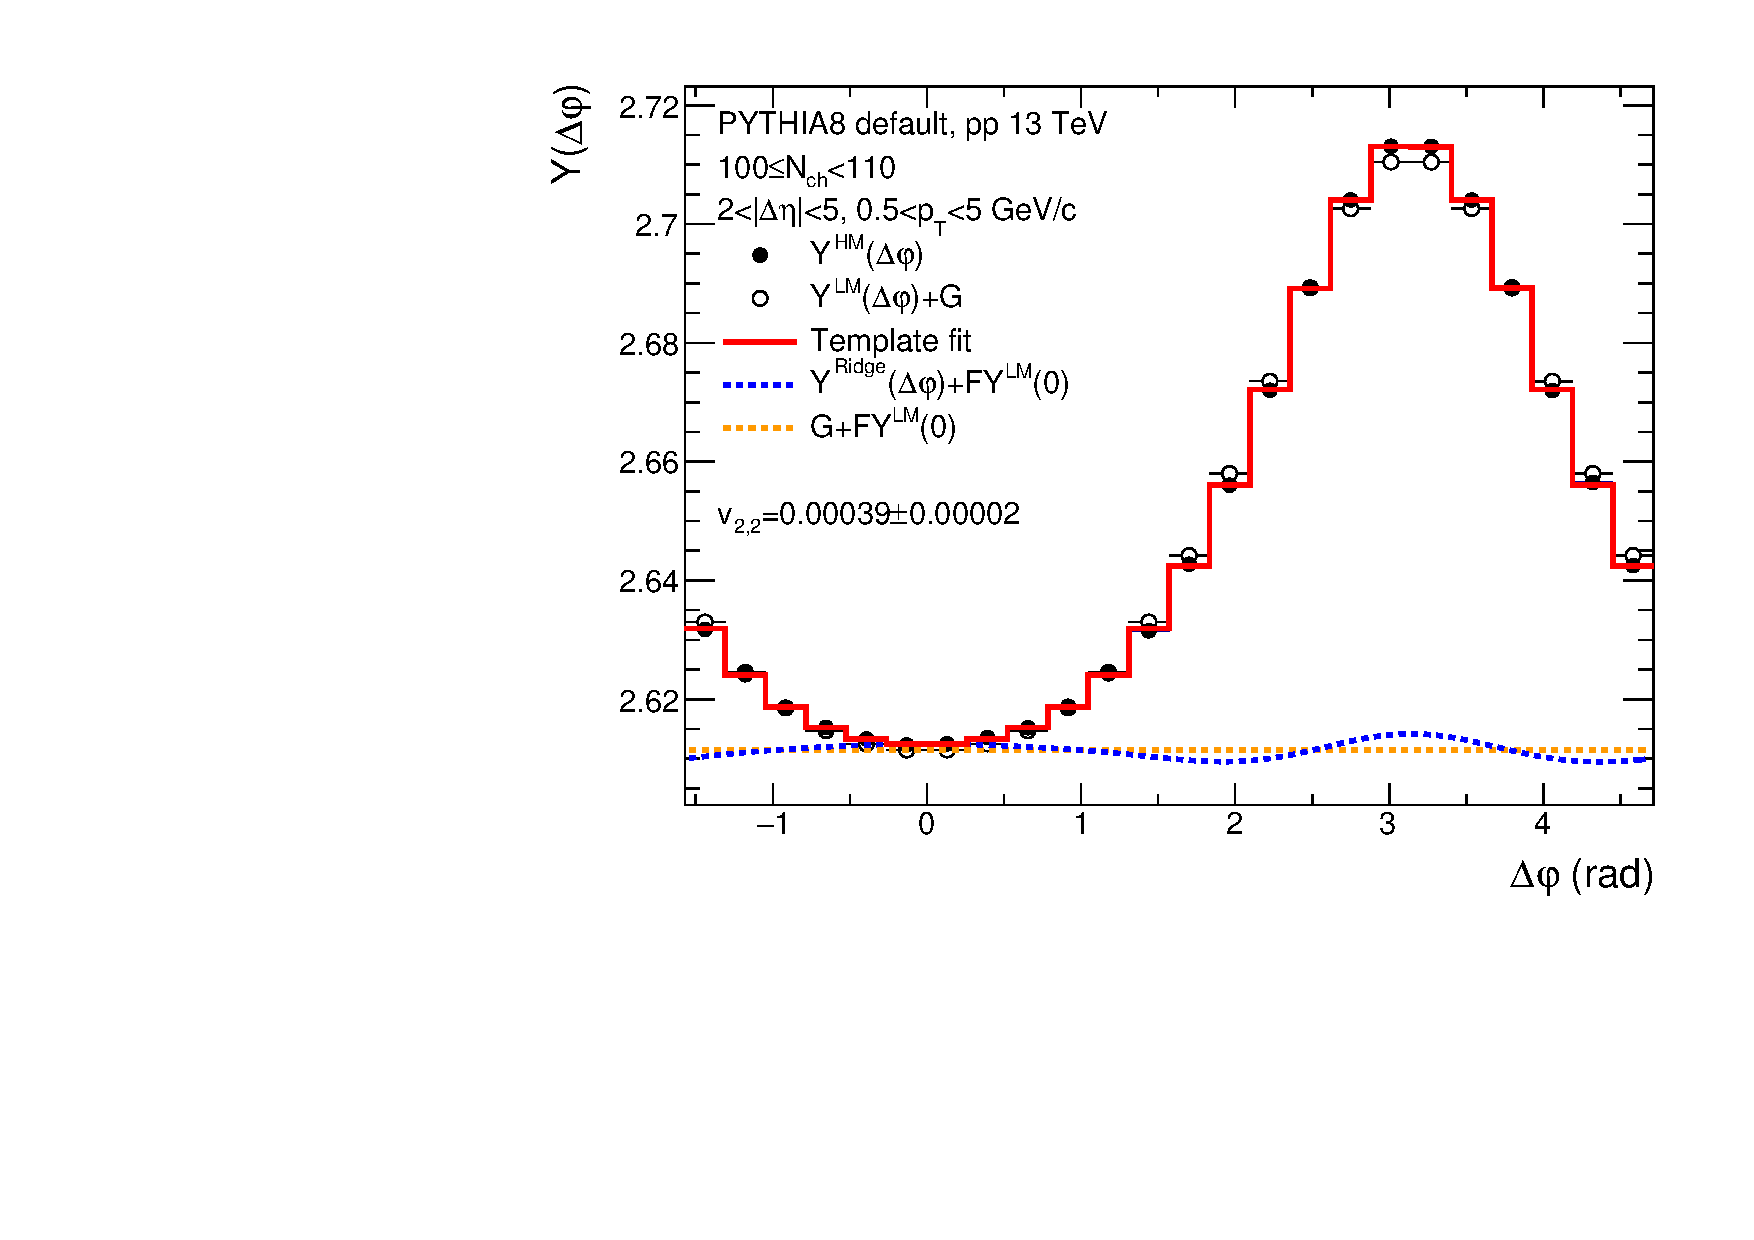
\includegraphics[width=0.49\textwidth]{figures/TemplateFit_default.pdf}
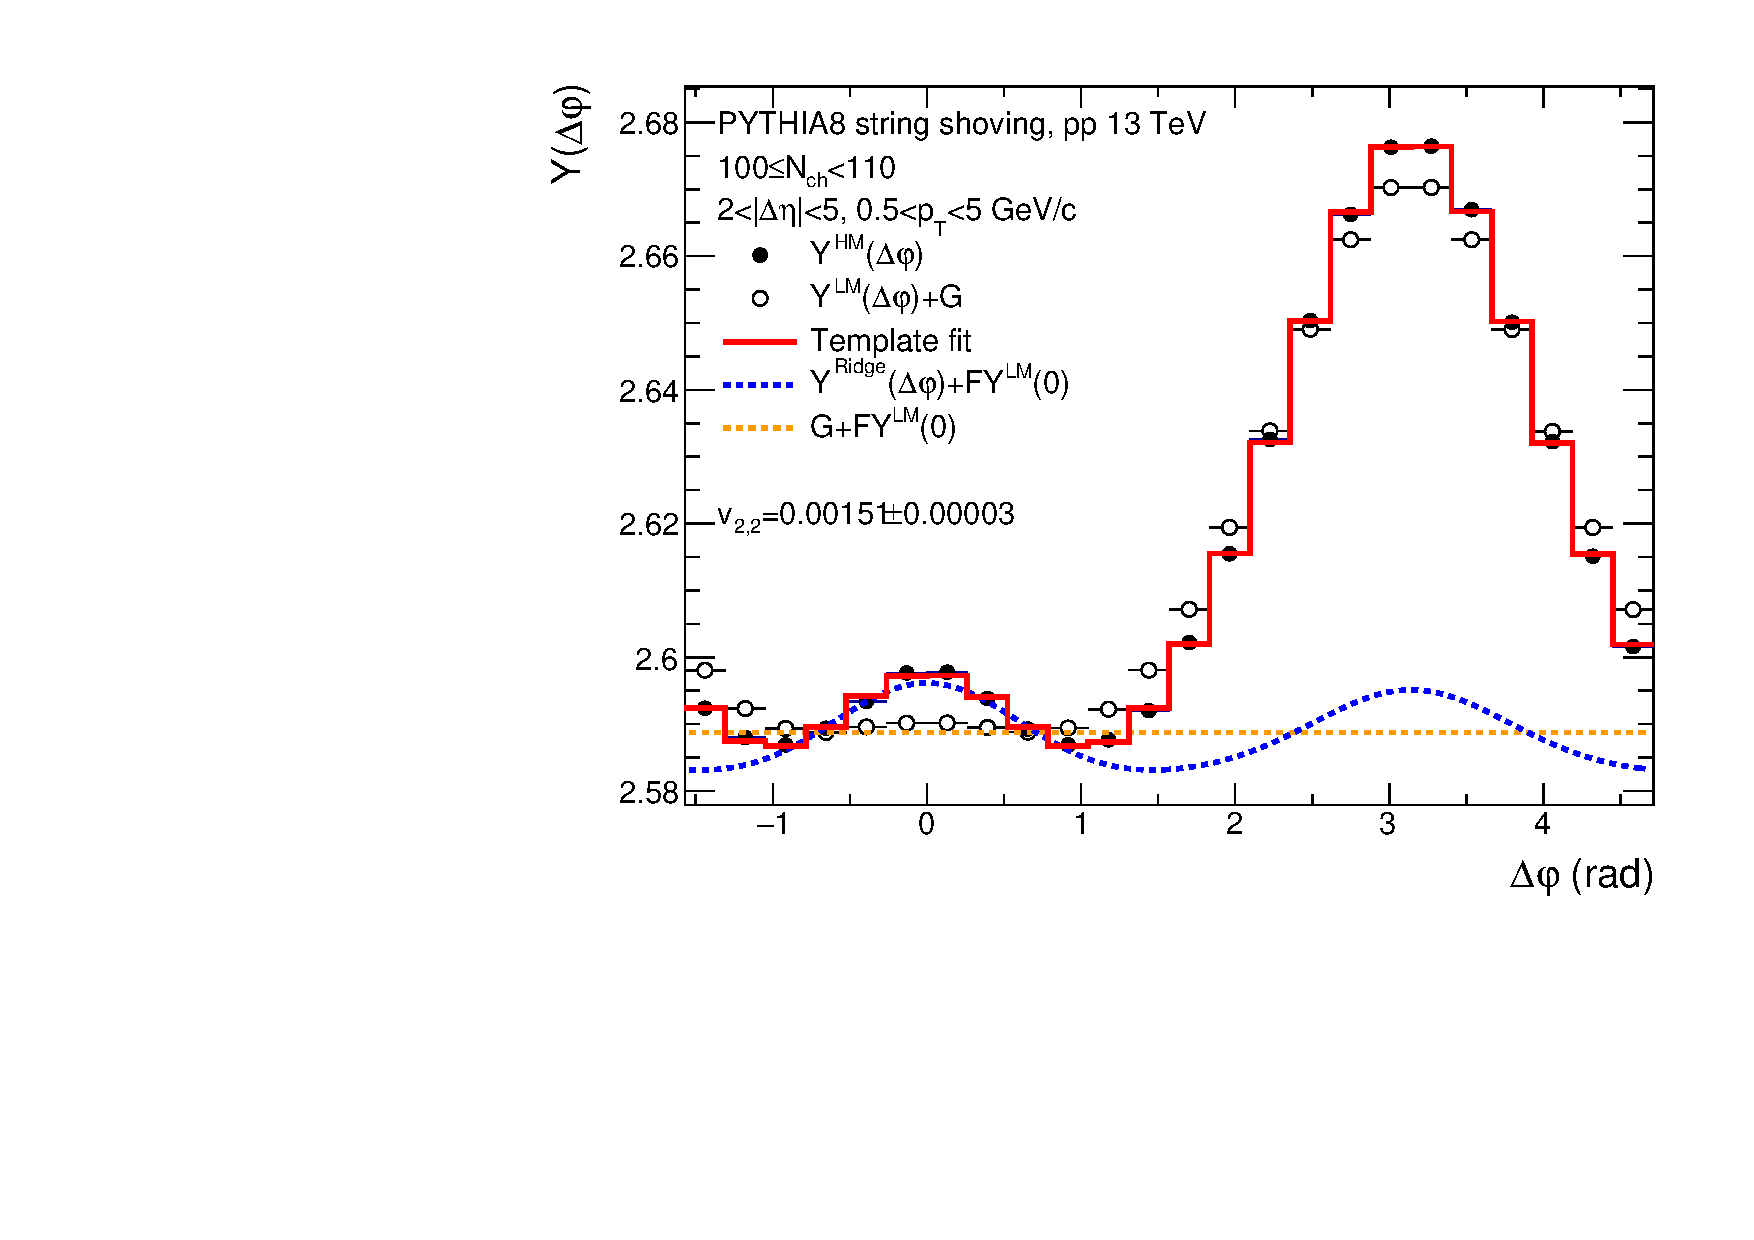
\includegraphics[width=0.49\textwidth]{figures/TemplateFit_shoving.pdf}
\caption{Template fits to one-dimensional correlation functions in high multiplicity ($100\leq\Nch<110$) \pythia events with the default configuration (left) and the string shoving model (right). The correlation function in low multiplicity ($0\leq\Nch<20$) events are used for the non-flow subtraction procedure.}
\label{fig:templatefit}
\end{figure}

In experiments, long-range two-particle correlations are also quantified with flow coefficients.
A template fit method developed by the ATLAS collaboration~\cite{Aad:2015gqa} to subtract non-flow effects is applied to \pythia events to obtain flow coefficients.
In the template fit method, correlation functions from low multiplicity events are used to estimate non-flow contributions:
\begin{align}
    Y^\mathrm{template}(\dphi) &= Y^\mathrm{ridge}(\dphi) + FY^\mathrm{LM}(\dphi),\nonumber\\
    Y^\mathrm{ridge}(\dphi) &= G \left( 1 + \sum^{\infty}_{n=2} 2 v_{n,n} \cos(n\dphi) \right),
\end{align}
where $F$ is a scale factor for correlation functions in low multiplicity events, and $v_{n,n}$ is a coefficient related to the $n$-th order flow coefficient.
Based on the assumption of factorization of flow coefficients, $v_{n,n}$ from two-particle correlations between trigger particles of $p_\mathrm{T}^{a}$ and associated particles of $p_\mathrm{T}^{b}$ is $v_{n,n}(p_\mathrm{T}^{a}, p_\mathrm{T}^{b}) = v_{n}(p_\mathrm{T}^{a}, p_\mathrm{T}^{b})$.
More details on the template fit method can be found in Ref.~\cite{Aad:2015gqa}.

Figure~\ref{fig:templatefit} shows the example of the template fits to one-dimensional correlation functions of charged hadrons in $0.5<\pt<5.0~\mathrm{GeV}/c$ from high multiplicity \pythia \pp events with the default configuration (left) and the string shoving option (right).
In order to compare with the ATLAS results, slightly different selections are used for multiplicity ($|\eta|<2.5$ and $\pt>0.4~\mathrm{GeV}/c$) and long-range ($2<|\deta|<5$).
In case of the default configuration, the correlation function from high multiplicity events is well described by the scaled correlation function from low multiplicity events.
Hence, the obtained $v_{2,2}$ is very small.
With the string shoving model, a clear near-side structure is seen in the correlation function from high multiplicity events ($Y^\mathrm{HM}(\dphi)$).
However, there is also a near-side peak in the correlation function in low multiplicity events ($Y^\mathrm{LM}(\dphi)$), the scaled $Y^\mathrm{LM}(\dphi)$ take a part of the near-side correlation in $Y^\mathrm{HM}(\dphi)$.
Therefore, one can expect that the obtained $v_{n,n}$ from the template fit method will be smaller than the true $v_{n,n}$ at the same multiplicity range.


\begin{figure}[!h]
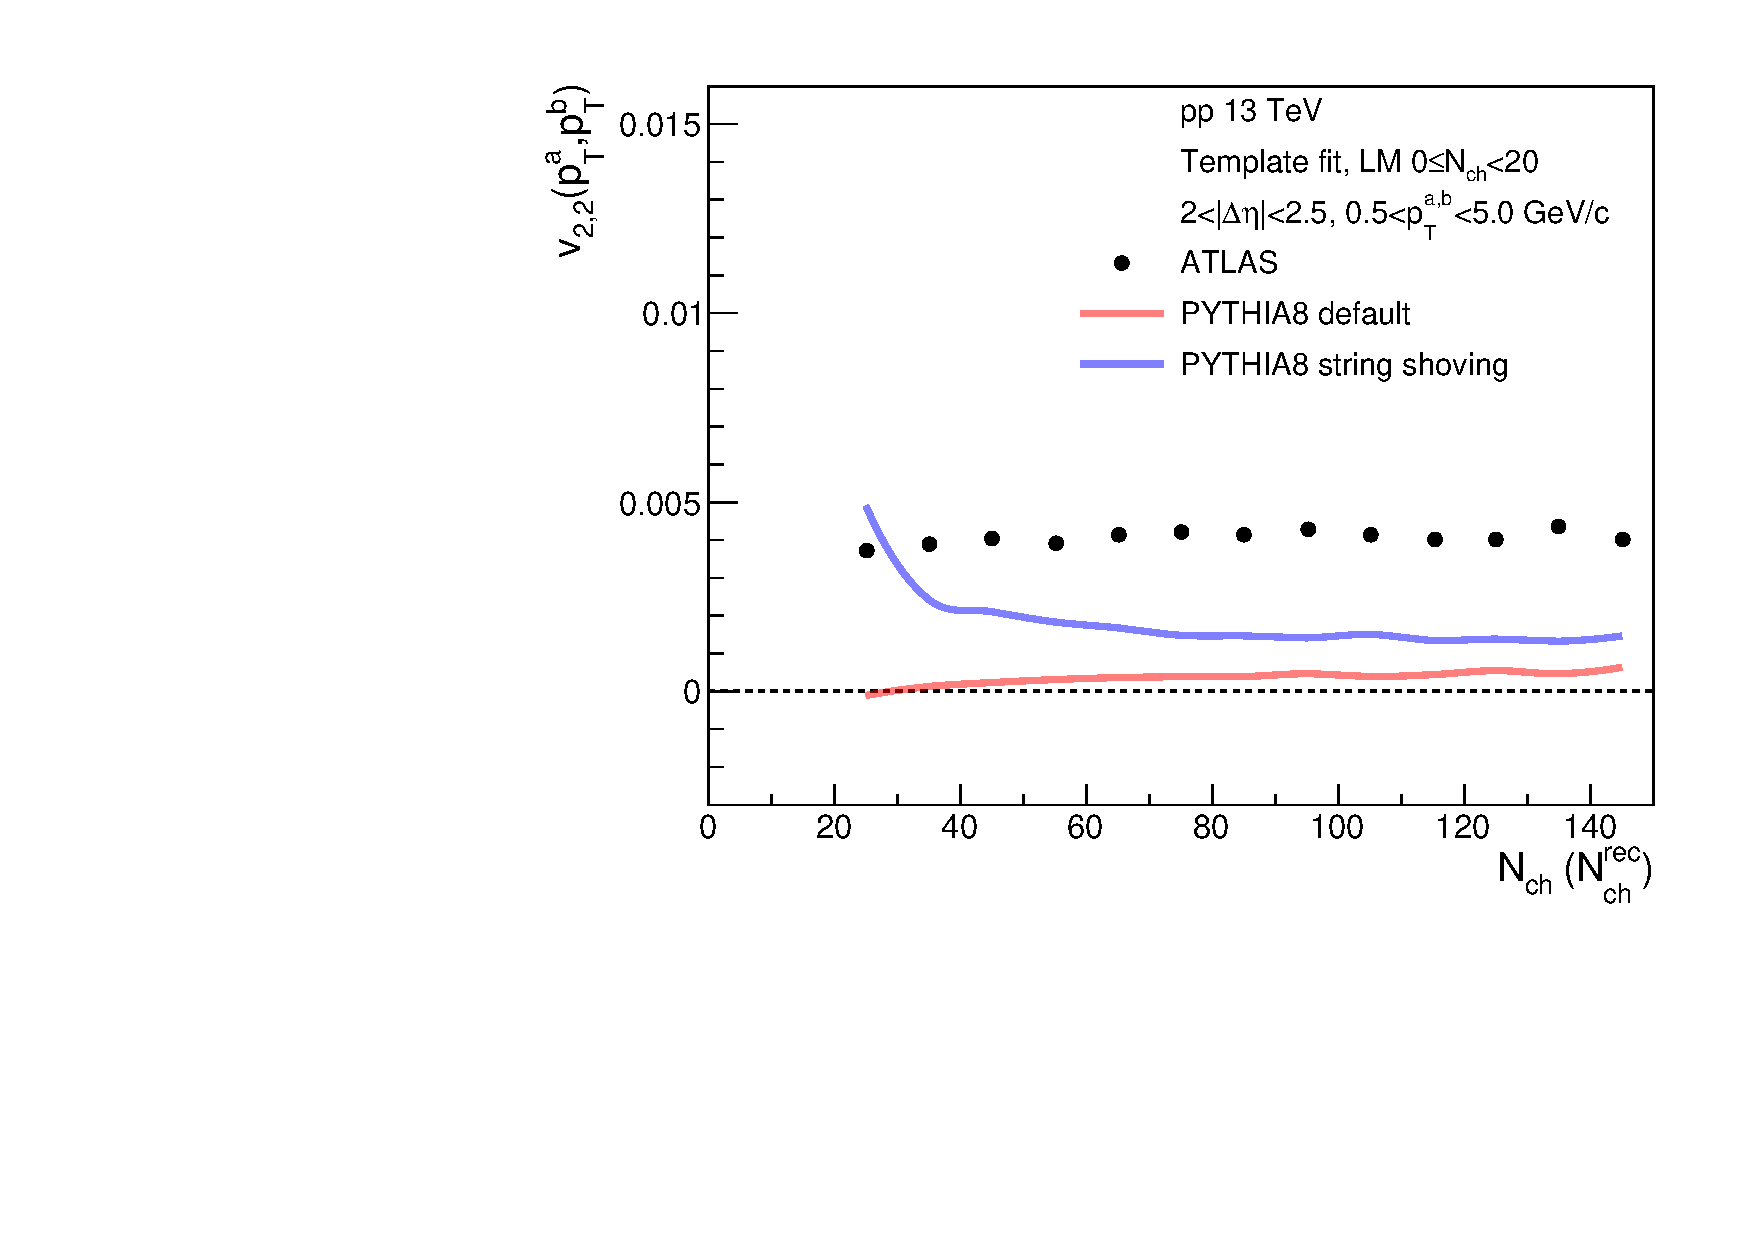
\includegraphics[width=0.49\textwidth]{figures/atlasmult.pdf}
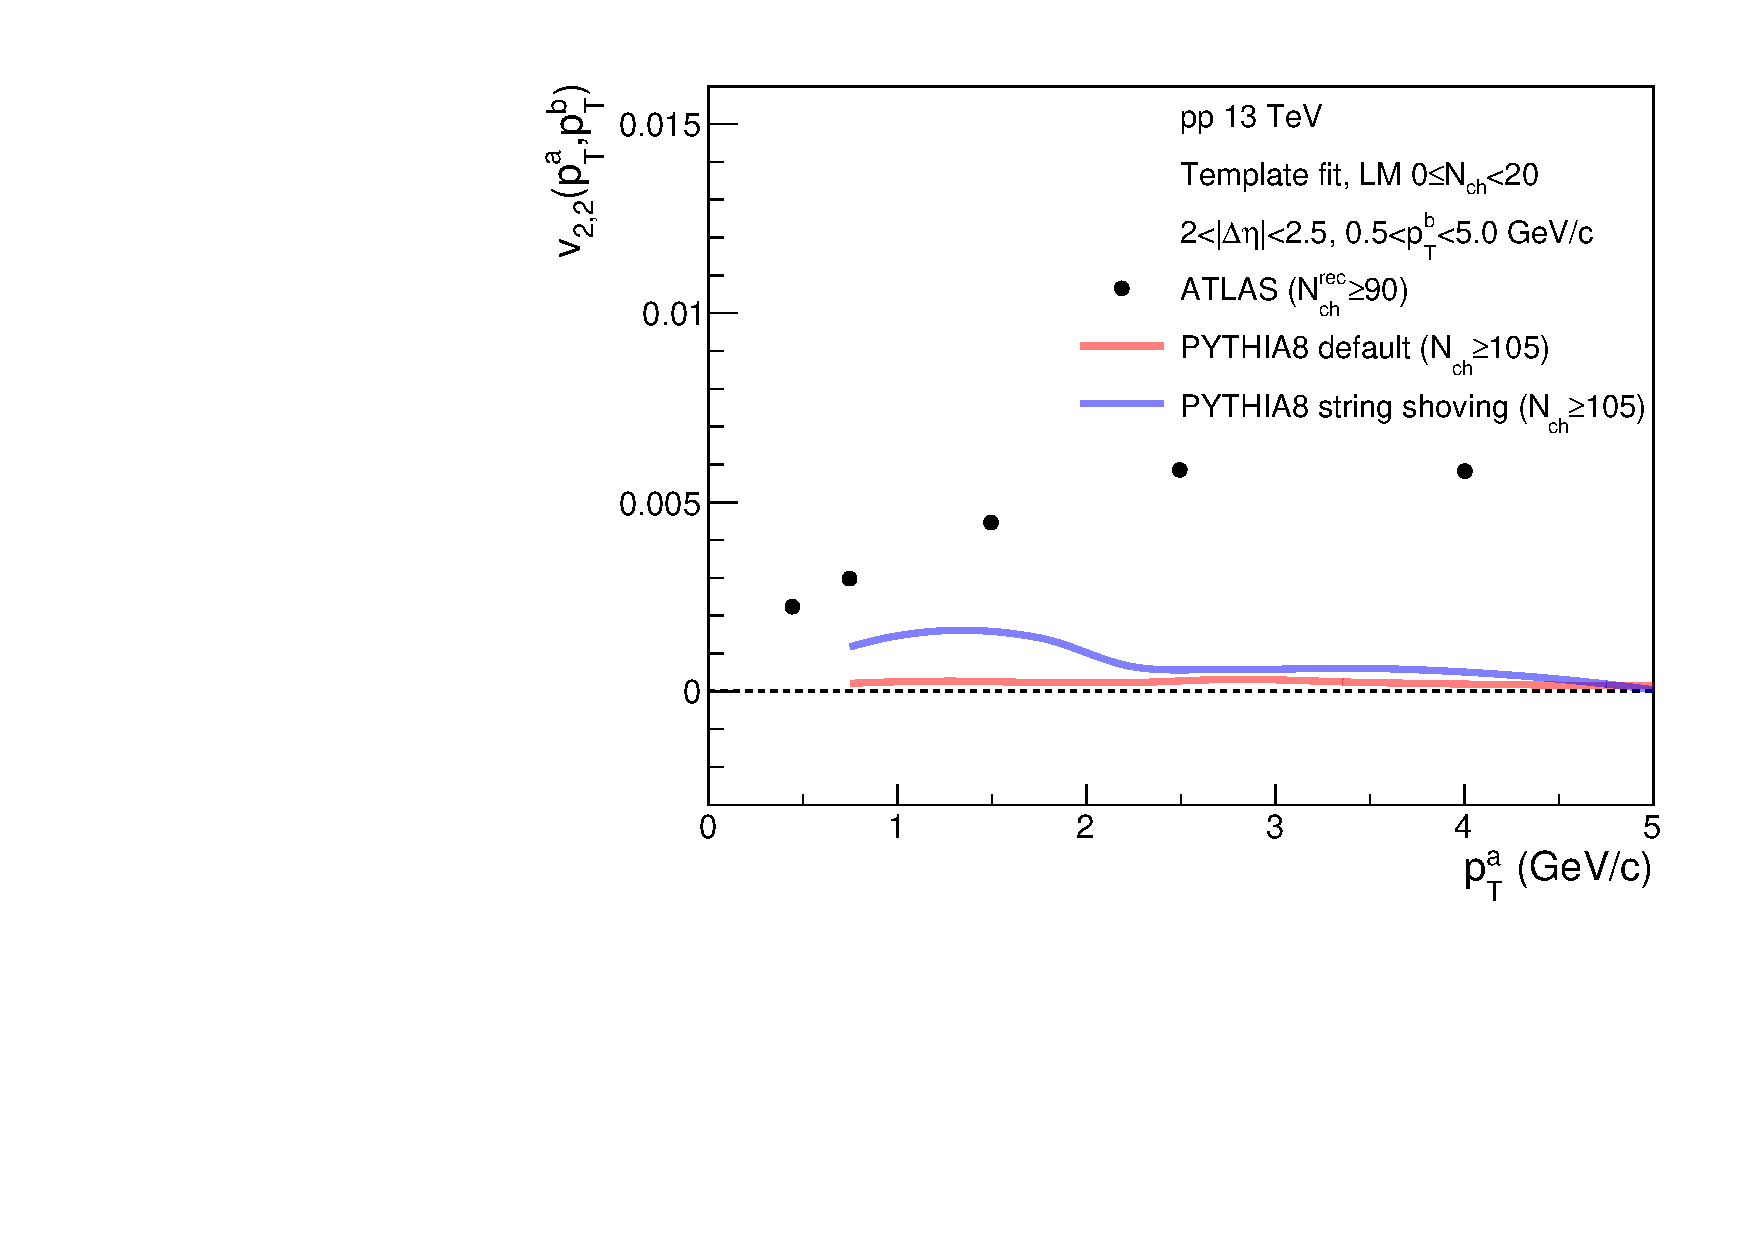
\includegraphics[width=0.49\textwidth]{figures/atlaspt.pdf}
\caption{$v_{2,2}$ obtained from the template fit method in \pythia events with the default configuration and the string shoving model, as a function of charged hadron multiplicity (left) and \pt (right). Results from \pythia events are compared with ATLAS results~\cite{Aad:2015gqa}.}
\label{fig:v22}
\end{figure}

%Flow modulations are extracted by subtracting back-to-back jets correlations at away-side in $\Delta\varphi$ correlations function. The subtraction method is implemented to remove back-to-back jets correlations mainly dominating away-side yield. The $\Delta\varphi$ correlations function measured in low-multiplicity event class is used for the subtraction procedure with the assumption that the ridge is negligible in low multiplicity event class, which is also observed in experiments. The template fitting procedure is achieved via
%\begin{eqnarray}
%Y(\Delta\varphi)=G \left\{ 1 + 2v_{2.2}\cos(2\Delta\varphi) + 2v_{3,3}\cos(3\Delta\varphi) \right\} + FY(\Delta\varphi)_{\rm{LM}}\quad.
%\end{eqnarray}
%Flow coefficients are denoted as $v_{2,2}$ and $v_{3,3}$ for elliptic and triangular modulation, respectively. $F$ is introduced to compensate the fact that jet yield measured in high multiplicity event class is higher than in low multiplicity event class, which results in under-subtraction of away-side yield with $F=1$.

Figure~\ref{fig:v22} shows extracted $v_{2,2}$ from the template fit method in \pythia events with the default configuration (red lines) and the string shoving model (blue lines) as a function of charged hadron multiplicity \Nch for charged hadrons in $0.5<\pt<5.0~\mathrm{GeV}/c$ (left) and as a function of \pt for high multiplicity events (right).
The $v_{2,2}$ from \pythia events with the default configuration are close to zero, and this demonstrates the non-flow subtraction method as the previous study in Ref.~\cite{Lim:2019cys}.
The results from \pythia events with the string shoving model show non-zero $v_{2,2}$ values which can be expected from long-range near-side correlation in the correlation functions.
In the comparison of the $v_{2,2}$ with ATLAS results~\cite{Aad:2015gqa}, the $v_{2,2}$ from the string shoving model is significantly lower than ATLAS results.
Based on the similar correlation functions in high multiplicity events shown in Figure~\ref{fig:dphi} and the over-subtraction of non-flow contribution shown in Figure~\ref{fig:templatefit}, the lower $v_{2,2}$ from the string shoving model is mainly due to the non-flow subtraction procedure with $Y^\mathrm{LM}(\dphi)$ showing a near-side peak.

%\begin{figure}[!h]
%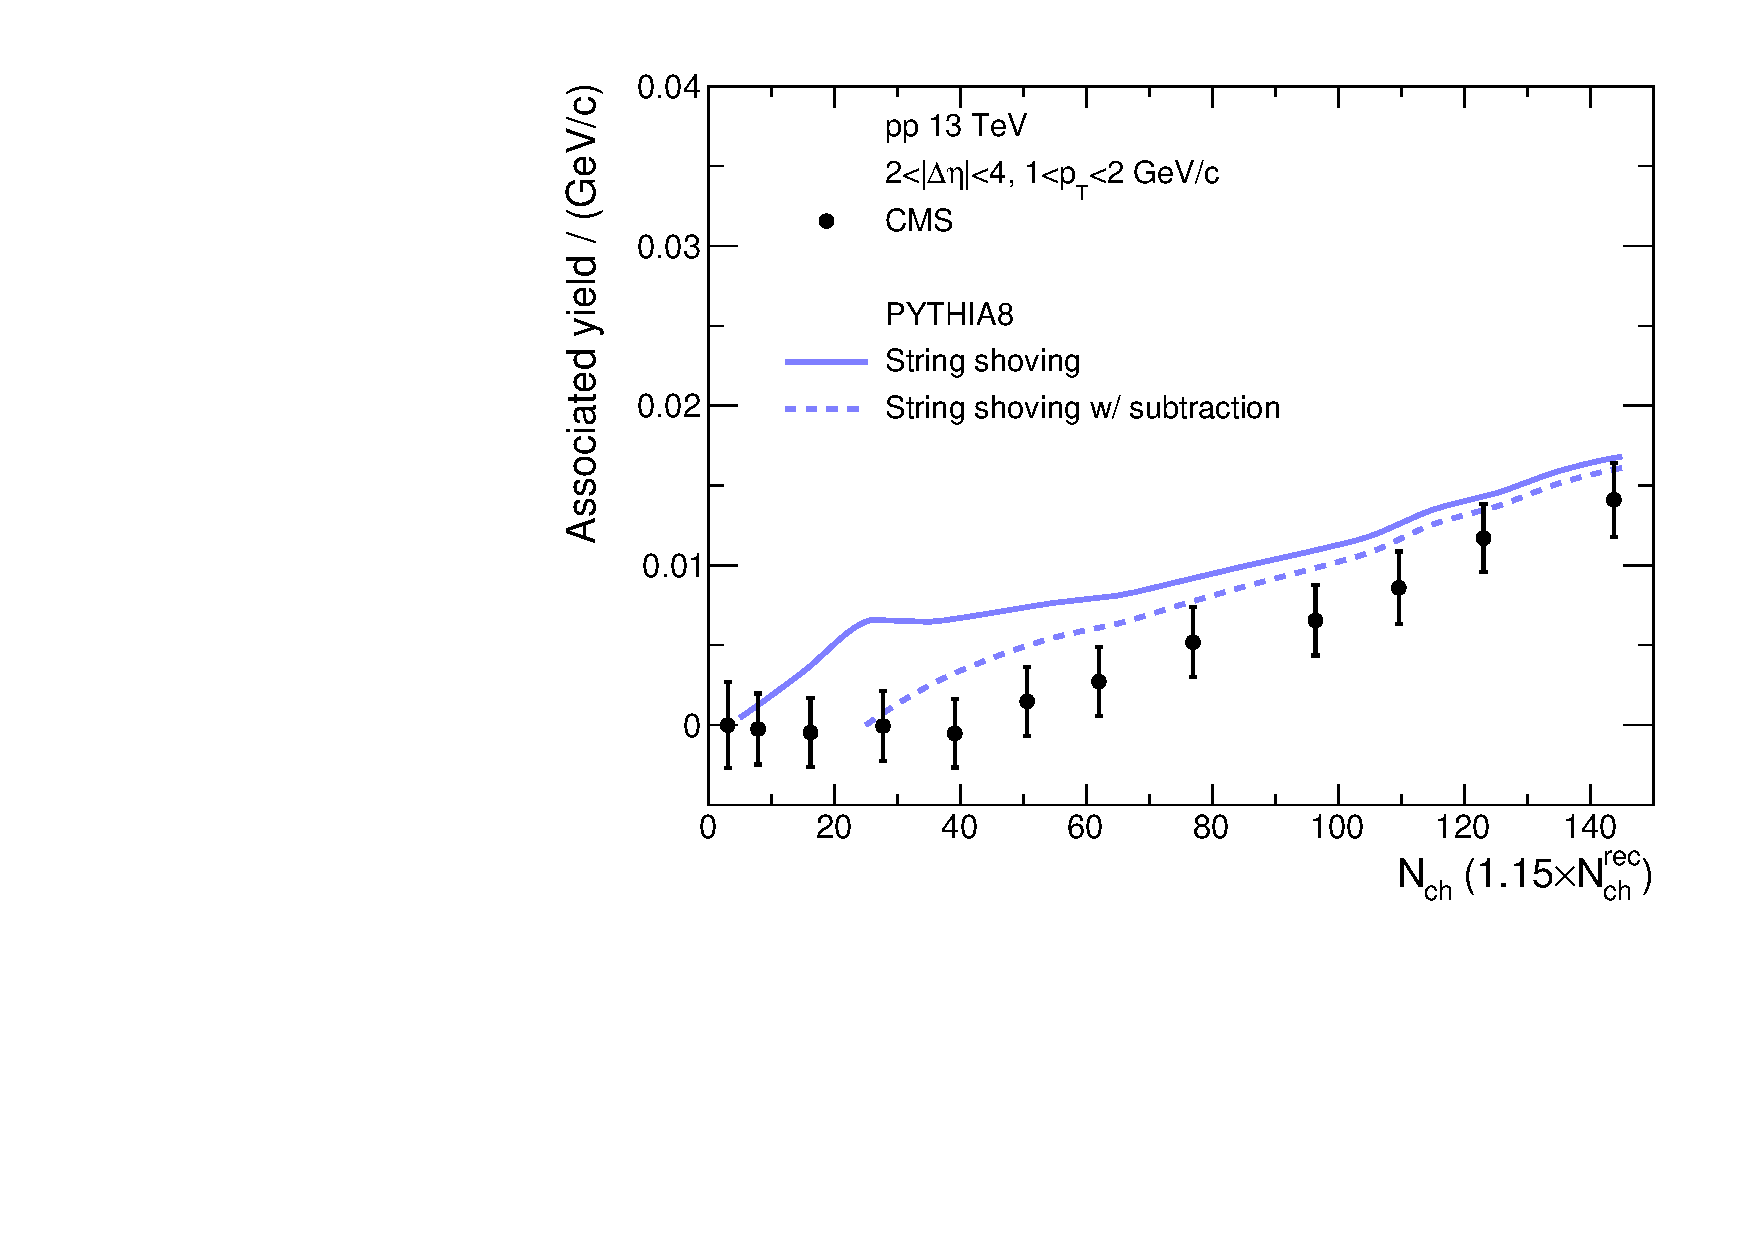
\includegraphics[width=0.49\textwidth]{figures/cmsmultSub.pdf}
%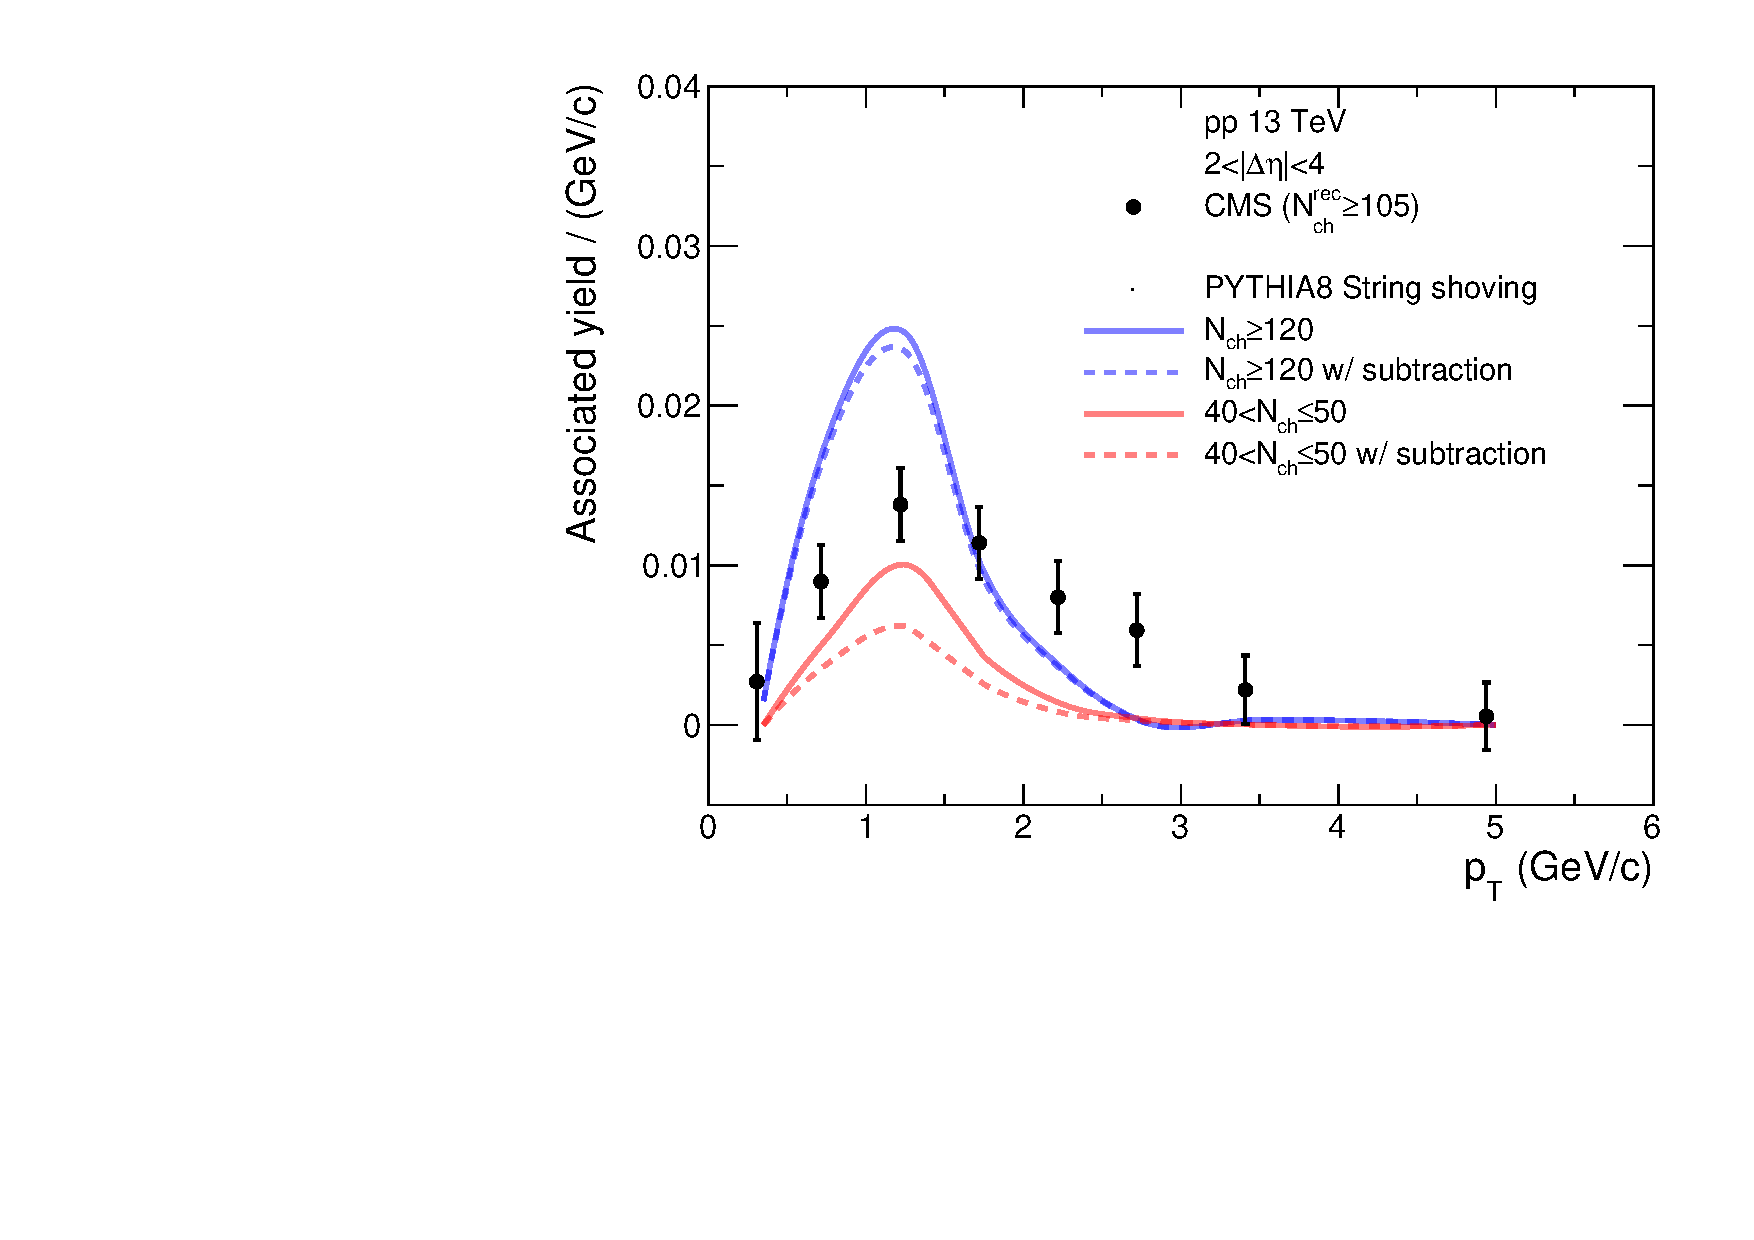
\includegraphics[width=0.49\textwidth]{figures/cmsptSub.pdf}
%\caption{(Associated yields of long-range near-side correlation functions as a function of \Nch for charged hadrons in $1<\pt<2~\mathrm{GeV}/c$ (left) and as a function of \pt for different multiplicity bins (right). Associated yields in $20<\Nch\leq 30$ are used for the subtraction procedure.}\label{fig:yasub}
%\end{figure}


